\documentclass[serif,mathserif]{beamer}
\usepackage{etex}
\usepackage{amsmath, amsfonts, epsfig, xspace}
\usepackage{algorithm,algorithmic}
\usepackage{pstricks,pst-node}
\usepackage{multimedia}
\usepackage[normal,tight,center]{subfigure}
\setlength{\subfigcapskip}{-.5em}
\usepackage{beamerthemesplit}
\usetheme{lankton-keynote}
\usepackage{graphicx,color}
% remove caption of figure
\usepackage[labelformat=empty]{caption}

\usepackage[none]{hyphenat} % hyphenation is ugly in slides
\usepackage{parskip}

\usepackage{relsize} % \smaller to change size

\usepackage{tikz}
\usetikzlibrary{calc}

\usetikzlibrary{arrows}

\newcommand{\TikzDraw}[2][]{
  \begin{tikzpicture}[overlay, remember picture, shift={(current page.center)}, #1]
    #2
  \end{tikzpicture}
}

\newcommand{\gridlines}{
  \TikzDraw{
    \draw[help lines,xstep=.2,ystep=.2,red!20] (current page.south west) grid (current page.north east);
    \draw[help lines,xstep=1,ystep=1,red] (current page.south west) grid (current page.north east);
    \foreach \x in {-15,-14,...,15} {
      \node [anchor=north, red] at (\x,0) {\tiny \x};
      \node [anchor=east,red] at (0,\x) {\tiny \x};
    }
  }
}

\newcommand{\DrawOnImg}[3][]
{
  \begin{tikzpicture}
    \node[anchor=south west,inner sep=0] (image) at (0,0){
      #2
    };
    \begin{scope}[x={(image.south east)},y={(image.north west)}]
      \ifthenelse{\equal{#1}{grid}}
                 {\draw[color=blue, style=dashed] (0,0) grid[xstep=.1, ystep=.1] (1.0001,1.0001);}
                 {}
                 #3
    \end{scope}
  \end{tikzpicture}
}


\newcommand{\BOLD}[1]{\mathbf{#1}}
\newcommand{\BOLDG}[1]{\boldsymbol{#1}}
\newcommand{\PDIF}[2]{\frac{\partial #1}{\partial #2}}
\newcommand{\TODO}[1]{\textcolor{red}{#1}}
\newcommand{\TODOB}[1]{\textcolor{blue}{#1}}
\newcommand{\TODOG}[1]{\textcolor{green!50!black}{#1}}
\newcommand{\argmin}{\operatornamewithlimits{arg\min}}
\DeclareMathOperator{\tr}{tr}
\DeclareMathOperator{\cond}{cond}
\DeclareMathOperator{\ST}{s.t.}
\DeclareMathOperator{\diag}{diag}

\author[Jiong Chen]{Jiong Chen}

\title[\hspace{2em}\insertframenumber/\inserttotalframenumber]{Nonlinear Material Design Using Principle Stretches}

\date{March 24, 2017}

% \institute{Zhejiang University}

\begin{document}

\maketitle

\begin{frame}
  \frametitle{Rig-Space Dynamics}
  \begin{itemize}
  \item Rigging: rig parameters $\rightarrow$ rigged surface
    \begin{equation*}
      \BOLD{p} \mapsto \BOLD{s}(\BOLD{p})
    \end{equation*}
    \pause
  \item Skeleton, cage, free-form deformation\dots
    \pause
  \item How to enrich the animation with physically plausible motion?
  \item
  \item
    \TikzDraw {
      \node at (-0.1, -2.6) {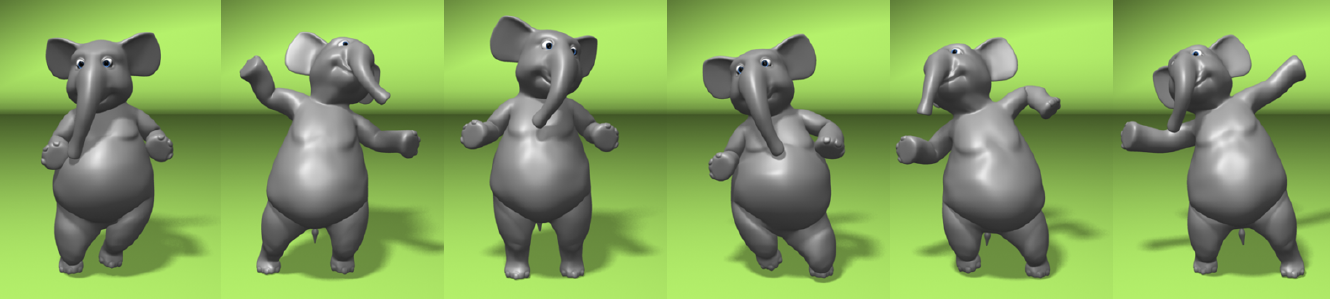
\includegraphics[width=0.9\textwidth]{img/elephant}};
    }
  \end{itemize}
\end{frame}

\begin{frame}
  \frametitle{Rig-Space Dynamics}
  \begin{itemize}
  \item Spatial discretization
    \begin{equation*}
      \BOLD{x} = \{\BOLD{n}\}\cup \{\BOLD{s}\}
    \end{equation*}
    \pause
  \item Lagrangian
    \begin{equation*}
      \begin{split}
        T &= \frac{1}{2}\BOLD{v_n}^T\BOLD{M_n}\BOLD{v_n} +\frac{1}{2}\BOLD{v_s}^T\BOLD{M_s}\BOLD{v_s}\\
        V &= W(\BOLD{n}, \BOLD{s}(\BOLD{p}))
      \end{split}
    \end{equation*}
    \pause
  \item Material for $W$?
  \end{itemize}
\end{frame}

\begin{frame}
  \frametitle{Impact of Material}
  \TikzDraw {
    \visible<1> {\node at (0, 0) {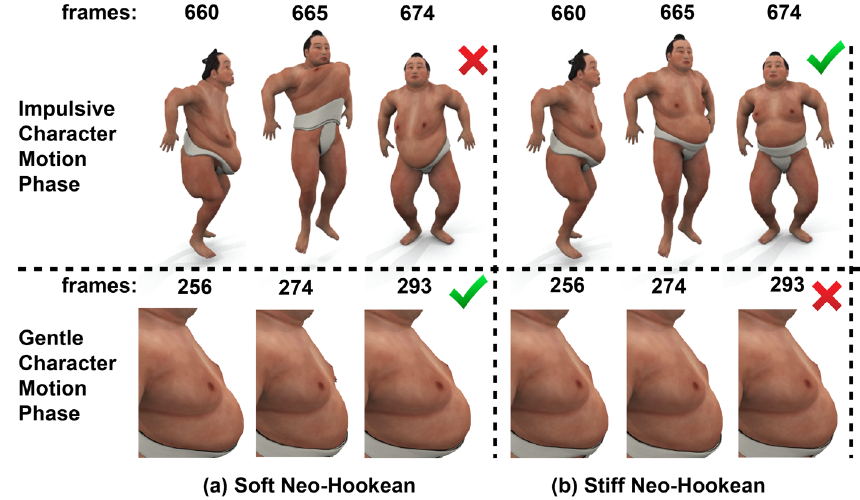
\includegraphics[width=\textwidth]{img/mtrartifact}};}
    \visible<2> {\node at (0, 0) {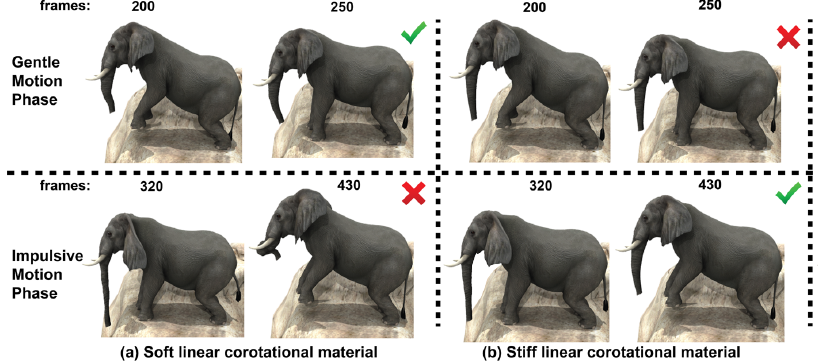
\includegraphics[width=\textwidth]{img/mtrartifact2}};}
  }
\end{frame}

\begin{frame}
  \frametitle{Expectation on Ideal Material}
  \begin{itemize}
  \item Yield soft behaviors around the rest state.
  \item Do not lead to excessive deformations for fast motion.
  \end{itemize}
  \TikzDraw {
    \visible<2-> {
      \node at (0, -1) {\TODO{\emph{How about naive stiffness adjustment?}}};
    }
  }
\end{frame}

\begin{frame}
  \frametitle{Background of Hyperelastic Material}
  \begin{itemize}
  \item Strain: 3D extension of $\Delta x$
    \begin{equation*}
      \BOLDG{\epsilon}_{green} = \frac{1}{2}(\BOLD{F}^T\BOLD{F}-\BOLD{Id}),~\BOLDG{\epsilon}_{coro} = \BOLD{S}(\BOLD{F})-\BOLD{Id},
    \end{equation*}
    \pause
  \item Isotropic Hook's law: 3D extension of $\frac{1}{2}k\Delta x^2$
    \begin{equation*}
      \Psi(\BOLD{F}) = \mu\|\BOLDG{\epsilon}\|_F^2 + \frac{\lambda}{2}\tr(\BOLDG{\epsilon})^2
    \end{equation*}
    \pause
  \item Stretch based expression by $F = U\Sigma V^T$
    \begin{equation*}
      \begin{split}
        &\Psi_{coro} = \mu(\sigma_1-1)^2+\mu(\sigma_2-1)^2+\frac{\lambda}{2}(\sigma_1+\sigma_2-2)^2 \\
        &\Psi_{stvk} = \frac{\mu}{4}(\sigma_1^2-1)^2+\frac{\mu}{4}(\sigma_2^2-1)^2+\frac{\lambda}{8}(\sigma_1^2+\sigma_2^2-2)^2 
      \end{split}
    \end{equation*}
  \end{itemize}
\end{frame}

\begin{frame}
  \frametitle{Numerical Issues}
  \begin{itemize}
  \item Force and tangent stiffness matrix computations.
    \pause
  \item Invariants of strain $\BOLD{C} = \BOLD{F}^T\BOLD{F}$
    \begin{equation*}
     \begin{split}
      &I_C = \tr(\BOLD{C}) =  \sigma_1^2+ \sigma_2^2 \\
      &II_C = \det(\BOLD{C}) = \sigma_1^2\sigma_2^2
     \end{split}
    \end{equation*}
    \pause
  \item This paper adopts SVD and its gradient.
  \end{itemize}
\end{frame}

\begin{frame}
  \frametitle{Benefits}
  \begin{itemize}
  \item Improvement on stability and performance
    \begin{figure}
    \centering
    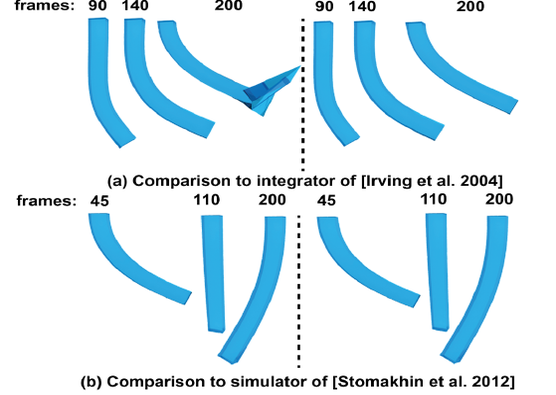
\includegraphics[width=0.5\textwidth]{img/svdgradbenefitAB}
    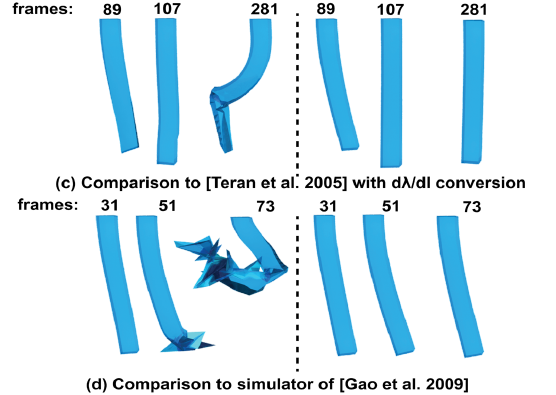
\includegraphics[width=0.5\textwidth]{img/svdgradbenefitCD}
  \end{figure}
  \end{itemize}
\end{frame}

\begin{frame}
  \frametitle{General Elastic Material Design}
  \begin{itemize}
  \item Isotropic material
    \begin{equation*}
      \Psi(\sigma_1, \sigma_2, \sigma_3) = \Psi(\sigma_{i_1}, \sigma_{i_2}, \sigma_{i_3})
    \end{equation*}
    \pause
  \item Valanis-Landel Hypothesis
    \begin{equation*}
      \boxed {
      \begin{split}
        \Psi(\sigma_1, \sigma_2, \sigma_3) = &f(\sigma_1)+f(\sigma_2)+f(\sigma_3) + \\
        &g(\sigma_1\sigma_2)+g(\sigma_2\sigma_3)+g(\sigma_3\sigma_1) + \\
        &h(\sigma_1\sigma_2\sigma_3)
      \end{split}
      }
    \end{equation*}
    \pause
  \item Stability condition
    \begin{equation*}
      \begin{split}
        \visible<3> {&d\BOLDG{\sigma} : d\BOLDG{\epsilon} \ge 0 \quad \text{[Drucker 1957]}} \\
        \visible<4> {&\frac{\partial^2 \Psi}{\partial \sigma^2} \text{~is always positive definite}\\}
      \end{split}
    \end{equation*}    
  \end{itemize}
  \TikzDraw {
    \visible<5> {
      \node at (0.5, -2.75) {\TODO{$\boxed{h(x) = g(x) = 0\Rightarrow f''(x) > 0 \Rightarrow f'(x) \nearrow}$}};
    }
  }
\end{frame}

\begin{frame}
  \frametitle{Material Editing by $f'$ Curve}
  \begin{itemize}
    \visible<1-> {
    \item Samples
      \begin{equation*}
        (x_k, f'(x_k)),~x_k \in [\sigma_{min}, \sigma_{max}]
      \end{equation*}
    }
    \visible<2-> {\item Fitting approach by
    \begin{equation*}
      \Psi_{ogden} = \sum_{p=1}^N \frac{\mu_p}{\alpha_p} (\sigma_1^{\alpha_p}+\sigma_2^{\alpha_p}+\sigma_3^{\alpha_p})
    \end{equation*}}
    \visible<4> {\item B\'ezier Spline
      \begin{equation*}
        \begin{split}
      f' &= \begin{bmatrix}
        \zeta^3 & \zeta^2 & \zeta &1
      \end{bmatrix}
      \begin{bmatrix}
        -1 & 3 & -3 &-1 \\
        3  & -6 & 3 & 0 \\
        -3  & 3 & 0 & 0 \\
        1  & 0 & 0 & 0
      \end{bmatrix}
      \begin{bmatrix}
        x_k \\
        a_k \\
        b_k \\
        x_{k+1}
      \end{bmatrix} \\
      \zeta &=(\sigma-x_k)/(x_{k+1}-x_k)
        \end{split}
    \end{equation*}}
  \end{itemize}
  \TikzDraw {
    \visible<1> {
      \node at (0.5, 0) {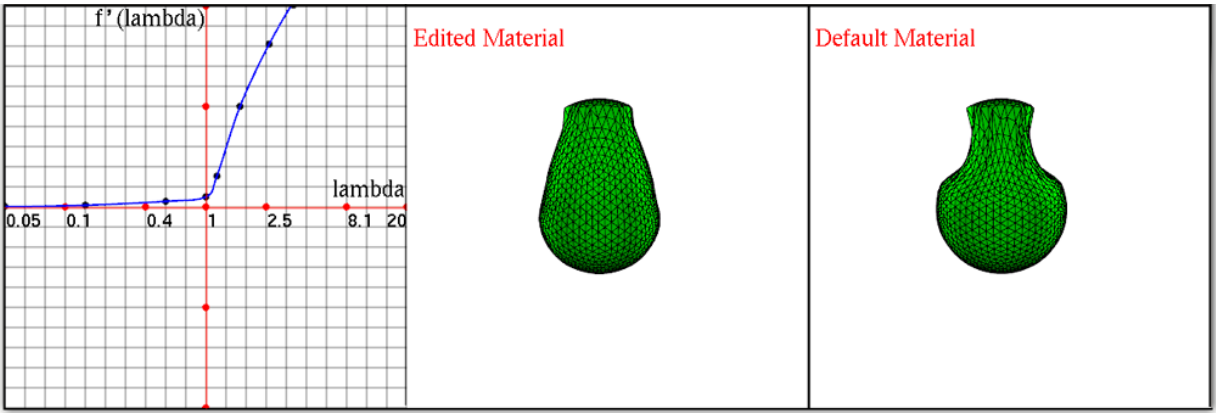
\includegraphics[width=0.8\textwidth]{img/designinterface}};
    }
    \visible<3> {
      \node at (0, -1) {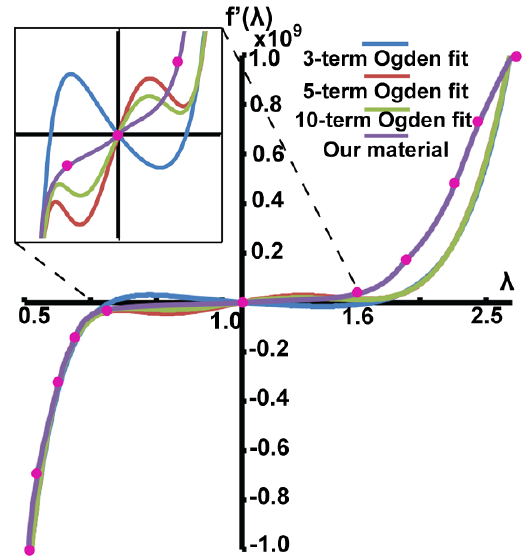
\includegraphics[width=0.5\textwidth]{img/ogden}};
    }
    \visible<5> {
      \node at (0.6, -2.2) {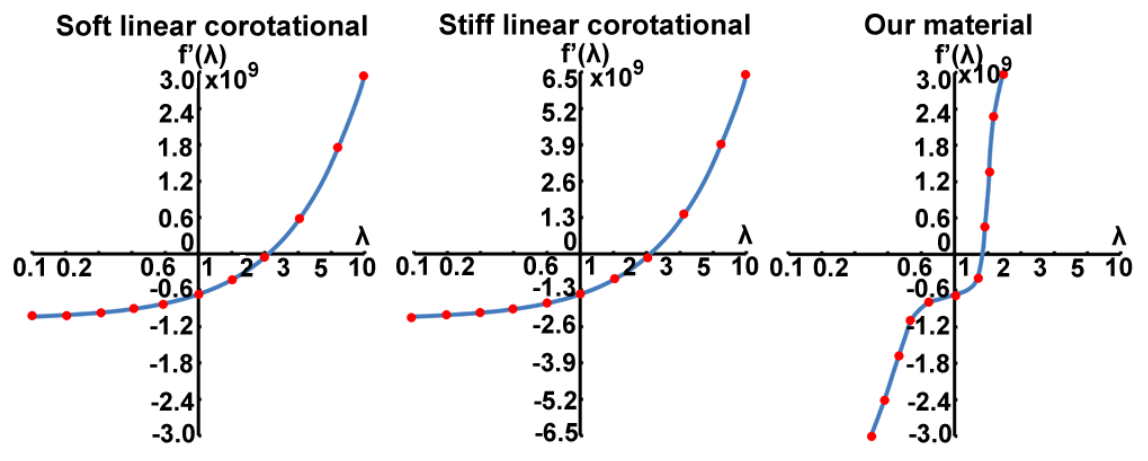
\includegraphics[width=0.8\textwidth]{img/editedmaterial}};
    }
  }
\end{frame}

\begin{frame}
  \frametitle{Material Editing by $f'$ Curve}
  \begin{itemize}
  \item Some tips for practice
    \begin{itemize}
    \item $f'$ curve is the most useful.
    \item Samples should increase in both $x$ and $y$ directions.
    \item Compression resistance term
      \begin{equation*}
        h +=
        \frac{\kappa}{12}(\frac{1-J}{6})^3\quad\text{if}~J < 1, \text{and}~0~\text{otherwise}.
      \end{equation*}
    \end{itemize}
  \end{itemize}
\end{frame}

\begin{frame}
  \frametitle{Anisotropic Case}
  \begin{itemize}
  \item Orthotropic nonlinear materials
    \begin{equation*}
      \begin{split}
        &\Psi = \Psi_{iso}(\sigma_1, \sigma_2, \sigma_3) + \Psi_{ortho} \\
        &\Psi_{ortho} =\sum_{i=1}^3 w_i(\|Fm_i\|_2)
      \end{split}
    \end{equation*}
  \end{itemize}
\end{frame}

\begin{frame}
  \frametitle{Results}
  
\end{frame}

\begin{frame} 
  \TikzDraw {
    \node at (0, 0.5) {\Huge{Thanks!}};
  }
  %\gridlines
\end{frame}


\end{document}
